% This is samplepaper.tex, a sample chapter demonstrating the
% LLNCS macro package for Springer Computer Science proceedings;
% Version 2.20 of 2017/10/04
%
\documentclass[runningheads]{llncs}
%
\usepackage{graphicx}
% Used for displaying a sample figure. If possible, figure files should
% be included in EPS format.
%
% If you use the hyperref package, please uncomment the following line
% to display URLs in blue roman font according to Springer's eBook style:
% \renewcommand\UrlFont{\color{blue}\rmfamily}
\usepackage{amsfonts}
\usepackage{wrapfig}
\usepackage{graphicx}
\usepackage{url}
\usepackage{cite}
\usepackage[dvipsnames]{xcolor}
\usepackage{algorithm}
\usepackage{algpseudocode}

\makeatletter
 \renewcommand{\ALG@name}{Algoritm}
\makeatother
\algrenewcommand\algorithmicfor{\textbf{pentru}}
\algrenewcommand\algorithmicdo{\textbf{execută}}
\algrenewcommand\algorithmicif{\textbf{dacă}}
\algrenewcommand\algorithmicthen{\textbf{atunci}}
\algrenewcommand\algorithmicend{\textbf{final}}
\algrenewcommand\algorithmicprocedure{\textbf{procedură}}
\algrenewcommand\algorithmicforall{\textbf{pentru fiecare}}

\begin{document}
%
\title{Cel mai mic strămoș comun}
%
%\titlerunning{Abbreviated paper title}
% If the paper title is too long for the running head, you can set
% an abbreviated paper title here
%
\author{Matei Barbu}
%
\authorrunning{Matei Barbu}
% First names are abbreviated in the running head.
% If there are more than two authors, 'et al.' is used.
%https://www.overleaf.com/project/5fad8e140b9466fcbf7974c2
\institute{Universitatea Politehnica București \\
Facultatea de Automatică și Calculatoare \\
\email{matei.barbu1905@stud.acs.upb.ro}}
%
\maketitle              % typeset the header of the contribution
%
\begin{abstract}
This paper presents a comparison between two classic algorithms, Tarjan-offline and RMQ, for the Lowest Common Ancestor problem. They are analyzed from the standpoint of time complexity, taking into account both phases of preprocessing and query answering. The comparison places focus not only on the reductibility of LCA to RMQ, but also on the flexibility of an established data structure, union-find.

\keywords{Algorithm \and Complexity \and Preprocess \and Query}
\end{abstract}
%
%
%
\section{Introducere}

\subsection{Descrierea problemei}

Dintr-un arbore cu rădăcină, $A = (V,E)$, din care alegem două noduri, $u,v \in V$, dorim să aflăm un nod, $w$, care este și strămoșul lui $u$ și al lui $v$. Dacă nodul $w$ are adâncime maximă atunci spunem că \emph{w este cel mai mic strămoș comun al lui u și v}. În decursul lucrării vom folosi și prescurtarea din engleză a problemei, lowest common ancestor, \emph{L.C.A.}, dar și \emph{C.M.M.S.C.} \\
Noțiunile de strămoș și adâncime vor fi folosite în sensul definițiilor de mai jos.

\renewcommand{\definitionname}{Definiția}
\begin{definition}
Lungimea unui lanț dintre două noduri este egală cu numărul de muchii ce unesc nodurile lanțului.
\end{definition}

\renewcommand{\definitionname}{Definiția}
\begin{definition}
Distanța cea mai scurtă dintre două noduri, $d : (V \times V) \to \mathbf{N}$.
$$d(u, v) =
\left\{
	\begin{array}{ll}
		\mbox{0}  & \mbox{dacă} \ x = y \\
		\mbox{min\{lungimea\ oricărui\ lanț\ dintre\ x, y\}}  & \mbox{dacă} \ x \neq y
	\end{array}
\right.
$$
\end{definition}


\renewcommand{\definitionname}{Definiția}
\begin{definition}
Adâncimea unui nod într-un arbore este egală cu distanța de la rădăcină la acel nod.
\end{definition}

\renewcommand{\definitionname}{Definiția}
\begin{definition}
Un nod $w$, este strămoș al lui $v$, dacă $w$ aparține lanțului de la rădăcina arborelui la $v$ și adâncimea lui $v$ este mai mare decât al lui $w$.
\end{definition}

\begin{wrapfigure}[12]{r}{0.15\textwidth}
    % \vspace{-30pt}
    \centering
    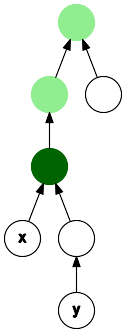
\includegraphics[width=0.15\textwidth]{LCA.png}
    \caption{~\cite{lca_poza}}
\end{wrapfigure}

\subsubsection{Exemplu:} Cel mai mic strămoș comun al lui x și y (vezi fig. 1) este colorat cu verde închis, iar toți strămoșii comuni sunt colorați verde deschis. Adâncimea lui x este 3, iar a lui y, 4.

\subsection{Aplicații practice}

\subsubsection{Genetica și taxonomia} sunt două domenii în care problema de față este utilă pentru a identifica trăsături comune în seturi de date sau contaminări culturale în genomuri. O implementare care utilizează direct C.M.M.S.C. este programul BASTA, despre care se pot citi mai multe în revista din referințe.~\cite{lca_taxonomie}

\subsubsection{Moștenirea claselor în programarea orientată pe obiecte} este un exemplu clasic în care este utilă determinarea relațiilor de dependență. O discuție pe tema determinării celei mai apropiate clase comune moștenită de două obiecte se află în referințe. ~\cite{lca_mostenire}

\subsection{Soluții propuse}

Cele două soluții alese pentru rezolvarea problemei sunt: algoritmul off-line al lui Tarjan și algoritmul de determinare cu ajutorul elementului minim dintr-un interval (R.M.Q. - Range Minimum Query).

În articolul din referințe de D. Harel și R. E. Tarjan, un contribuitor la importante rezultate legate de pădurile de mulțimi disjuncte, vezi ~\cite{CLRS} pag. 585, a fost printre primele studii importante pe această tema, în care au demonstrat că este necesară pentru un răspuns în timp constant o preprocesare liniară. ~\cite{Harel_Tarjan}

În ceea ce privește reducerea C.M.M.S.C. la E.M.I., adică la determinarea elementului minimului dintr-un interval, aceasta se poate face în timp liniar, deși aparent problemele nu sunt asemănătoare. E.M.I. se poate reduce la rândul lui la C.M.M.S.C. ~\cite{lca_algopedia} Implementarea soluției se va face prin metoda programării dinamice.

\subsection{Criterii de evaluarea a soluțiilor}

Algoritmii propuși se diferențiază în primul rând prin complexitățiile lor spațiale și temporale, dar mai ales prin modul de tratare a interogărilor. Algoritmul lui Tarjan necesită ca toate interogările să fie date în avans. Răspunsurile la întrebări se dau în timp ce procesăm graful, de aici și denumirea de \emph{off-line}. Abordarea online ne prezintă fiecare interogare doar după ce am răspuns la cea anterioară.

Astfel, în evaluarea teoretică a calității soluțiilor nu este suficientă caracterizarea printr-un singur termen, corespunzător complexității temporale asimptotice, ci trebuie să luăm în calcul, separate una de cealaltă, complexitatea preprocesării și cea a interogărilor. Spre deosebire, complexitatea spațială adițională va fi în general caracterizată de memoria structurii de date necesare etapei de preprocesare.

Testele vor încerca să sublinieze calitățile individuale ale fiecărui algoritm și mai ales să răspundă la următoarele întrebări: Ce soluție performează când avem un număr de interogări mic, respectiv mare? Este justificată memoria necesară preprocesării?

\section{Prezentarea soluțiilor}

\subsection{Modul de funcționare}

\subsubsection{Algoritmul lui Tarjan off-line} se bazează pe următoare observație ca să aflăm cel mai mic strămoș dintre un nod, \textcolor{blue}{\emph{x}}, pe care îl vom colora \textcolor{blue}{\emph{albastru}}, și orice alt nod, \emph{z}: pornim din z și urcăm din părinte în părinte, până când intersectăm \textcolor{ForestGreen}{lanțul}, \textcolor{ForestGreen}{verde}, de la \textcolor{blue}{\emph{x}}, la rădăcina, \textcolor{red}{\emph{r}}, \textcolor{red}{\emph{roșie}}, astfel nodul de intersecție este C.M.M.S.C., vezi fig. \ref{fig:tarjan_pic}. Ca să otimizăm această soluție brutală, pentru fiecare nod \textcolor{ForestGreen}{y}, \textcolor{ForestGreen}{verde}, de pe lanțul de la nodul \textcolor{blue}{\emph{x}} la \textcolor{red}{\emph{r}}, îi luăm fii lui \textcolor{ForestGreen}{y} și îi punem într-o nouă mulțime disjunctă dintr-o pădure al cărei strămoș îl marcăm \textcolor{ForestGreen}{y}. Astfel pentru orice nod z, negru, trebuie doar să aflăm care este strămoșul acelei mulțimi.

\begin{figure}
    \centering
    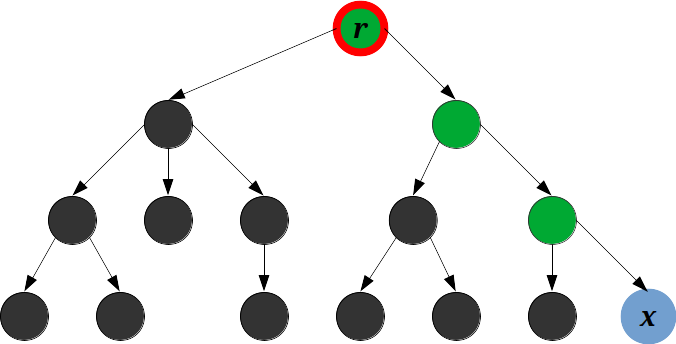
\includegraphics[width=7cm]{arbore_tarjan.png}
    \caption{Ideea din spatele algoritmului lui Tarjan}
    \label{fig:tarjan_pic}
\end{figure}

Pornim din rădăcina arborelui, o procedură recursivă, cf. alg. \ref{tarjan}, după cum este prezentat în referințe \cite{CLRS}, pag. 584. Pentru fiecare fiu al nodului curent procesează mulțimea disjunctă a fiului și răspunde la anumite interogări, iar apoi unește mulțimea fiului disjunctă cu cea a nodului curent. Pentru fiecare interogare care conține nodul curent și un alt nod vizitat deja, află strămoșul celuilalt nod. Vom reține o listă ascoiată fiecărui nod în care salvăm toate interorările în care acesta apare. Vom folosi implementarea de pădure de mulțimi disjuncte cu două euristici: reuniunea după rang și comprimarea drumurilor. Vezi \cite{CLRS} pag. 571-581.

\subsubsection{Algoritmul cu determinarea E.M.I.} se bazează pe următoarea observație, într-o parcurgere în adâncime a arborelui, între vizitele dintre două noduri, $u$ și $v$,  cel mai adânc nod vizitat este C.M.M.S.C. Deci, reducem problema la E.M.I. cu tehnica turului eulerian. Arborele este privit precum un graf orientat, între două noduri vecine inserându-se două arce orientate diferit. Se pornește din tatăl arborelui și se parcurge graful mai în adâncime, inserându-se tatăl în tur după fiecare fiu vizitat. Vezi alg \ref{tur_eulerian}. La final vom avea $2N-1$ noduri în tur, dat de numărul de noduri, adică $N$, plus numărul de arce incidente fiecărui tată, adică, $N-1$.

Pe reprezentarea vectorială a turului eulerian, $tur$, o să observăm că pentru două noduri, $v$ și $u$, care au prima apariție în $tur$, $i$, respectiv $j$, cu $i \leq j$, cel mai mic strămoș comun al lor este nodul dintre $i$ și $j$ cu adâncimea minimă.

Vom determina E.M.I. cu tehnica programrii dinamice, folosind un tabel rar, având $N$ noduri în arborele inițial, pentru $0 \leq i \leq 2(N - 1)$ și $0 < j \leq [log_2(N)]$, vom reține în tabel:

\emph{t(i)(j) = cel mai mic adânc nod din subsecvenţa tur(i, i + $2^j$ – 1)}

Vom folosi următoarea recurență pentru a genera tabelul:

$$ t(i, j) =
\left\{
	\begin{array}{ll}
	    \mbox{$tur(i)$} & \mbox{dacă} \ j = 0 \\
		\mbox{$t(i,j - 1)$} & \mbox{dacă $nivel(t(i, j - 1)) < nivel(t(i + 2^{j-1}, j - 1))$} \\
		\mbox{$t(i + 2^{j-1}, j - 1)$}  & \mbox{altfel}
	\end{array}
\right.
$$

Deci pentru a afla C.M.M.S.C. dintre $u$ și $v$, care au prima apariție în $tur$, $i$, respectiv $j$, cu $i \leq j$, iar $len = j - i + 1$, și $l_2 = log_2(len)$

$$ CMMSC(u, v) =
\left\{
	\begin{array}{ll}
	    \mbox{$t(i, l_2)$} & \mbox{dacă $nivel(t(i, l_2)) < nivel(t(j-2^{l_2} + 1, l_2))$}\\
		\mbox{$t(j-2^{l_2} + 1, l_2)$}  & \mbox{altfel}
	\end{array}
\right.
$$

\subsection{Analiza complexitații soluțiilor}

\subsubsection{Algoritmul lui Tarjan} îl vom analiza pas cu pas. 

Operația \emph{formează\_mulțime} are complexitatea amortizată $\Theta(1)$, cf. \emph{lemei 21.11}, pag. 579, \cite{CLRS}.

Operația \emph{găsește\_mulțime} are complexitatea amortizată $O(\alpha(N))$, cf. lemei 21.13, pag. 580, \cite{CLRS}, unde $\alpha$ este inversa funcției lui Ackermann.

Operația \emph{unește} are complexitatea amortizată $O(\alpha(N))$, deoarece doar apelează la rândul său în spate două operații de tip \emph{găsește\_mulțime}, și apoi execută o reuniune după rang în $\Theta(1)$.

Operația \emph{marchează\_strămoș} are complexitatea amortizată $O(\alpha(N))$, deoarece doar apelează la rândul său în spate două operații de tip \emph{găsește\_mulțime}. Apoi execută operații cu cost $\Theta(1)$.

Astfel, complexitatea \textbf{temporală} amortizată a \textbf{preprocesării} din alg. \ref{tarjan}, liniile 1-8, este dată de operațiile de mai sus din parcurgerea în adâncime, deci $O(N\alpha(N))$. Complexitatea \textbf{spațială} a preprocesării este $\Theta(N)$, deoarece folosim doar doi vectori pentru reprezentarea taților și a rangurilor.

Pentru fiecare din cele $M$ interogări, se efectuează o operație de \emph{găsește\_mulțime}, aceasta însemnând o complexitate \textbf{temporală} amortizată pentru toate răspunsurile de $O(M\alpha(N))$. Complexitatea \textbf{spațială} pentru răspunsuri este $\Theta(M)$, deoarece folosim câte o listă pentru fiecare nod, cu interogările care îl conțin, și doar un vector de răspunsuri.

\subsubsection{Algoritmul cu determinarea E.M.I.}  îl vom analiza pas cu pas.

Pentru a precalcula turul eulerian vom avea nevoie de $\Theta(N)$, \textbf{timp} deoarece avem doar de făcut o parcurgere în adâncime într-un arbore, care are $N-1$ muchii. În ceea ce privește \textbf{memoria}, compexitatea este $\Theta(N)$, deoarece vom avea în final $2N-1$ noduri în tur, iar vectorii de reținere a adâncimii și a primei apariții a unui nod în tur, aparțin aceleași clase de complexitate, $\Theta(N)$.

Pentru a precalcula tabelul vom avea nevoie de $\Theta(Nlog(N))$ \textbf{memorie} și \textbf{timp}, din motivele specificate când am definit recurența de generare.

Pentru fiecare din cele $M$ interogări, vom răspunde în $\Theta(1)$, deoarece determinarea C.M.M.S.C. se face doar din instrucțiuni de decizie, cum am specificat mai sus. Deci în total $\Theta(M)$ timp de răspuns, și precum această soluție poate funcționa \emph{on-line}, ne putem lipsi de stocarea interogărilor.

\subsection{Avantaje și dezavantaje}

\subsubsection{Algoritmul lui Tarjan} are principalul avantaj că folosește doar $\Theta(N)$ memorie adițională pentru precalcul. Deși inversa funcției lui Ackermann crește \textbf{foarte lent}, constantele de timp din acest algoritm nu sunt neglijabile în practică, când avem \textbf{multe} interogări.

\subsubsection{Algoritmul cu determinarea E.M.I.} are principalul avantaj că răspunde instant la interogări fără memorie adițională pentru ele. Dezavantajul se materializează într-un cost mai mare de memorie și timp pentru precalcul, când avem \textbf{puține} interogări.

\section{Evaluare}

\subsection{Proiectarea testelor}

Mai întâi am folosit testele de pe site-ul din referințe \cite{infoarena_teste}, pentru a verifica corectitudinea implementărilor.

Apoi, am scris un script Octave, care primește numărul de noduri și interogări, și generează folosind o bibliotecă de numere pseudo-aleatore fișierele de intrare. Pentru vectorul de tați, pe poziția $i$, am generat un tatăl, $t$, respectând relația, $t < i$. Astfel se evită ciclurile. Interogările sunt generate complet aleator.

\subsection{Specificațiile sistemului de evaluare}

\texttt{
\begin{tabbing}
System:\ \ \ \ \=Host: Kernel: 4.19.0-13-amd64 x86\_64 bits: 64 \\
         \> base: Debian 10.2 buster \\
         \> compiler: gcc v: 8.3.0 \\
CPU:     \> Topology: Quad Core model: Intel Core i7-8550U bits: 64 \\
         \> cache: 8192 KiB \\
Graphics:\> Intel UHD Graphics 620 \\
Memory:  \> 16GB type: DDR4 \\
Disk:    \> type: SSD
\end{tabbing}
}

\subsection{Ilustrarea rezultatelor}

Pentru fiecare din testele de pe infoarena am realizat un grafic care ilustreaza secundele de rulare.

\begin{figure}
    \centering
    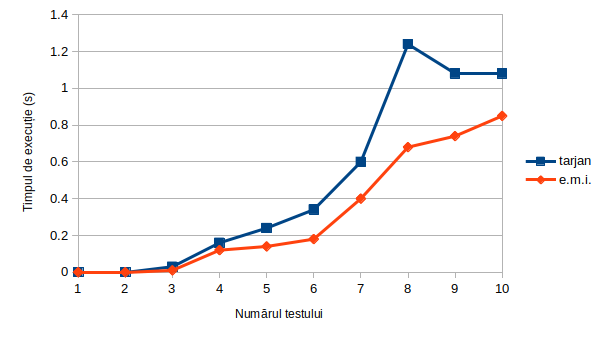
\includegraphics[width=10cm]{infoarena.png}
    \caption{Performanță pe testele de corectitudine}
    \label{infoarena_teste_poza}
\end{figure}

În ceea ce privește testele proprii le-am dat următoarele dimensiuni:

\begin{center}
 \begin{tabular}{||c c c||} 
 \hline
 Nr. test & N & M \\
 \hline\hline
 0 & $10^3$ & $10^6$ \\ 
 \hline\hline
 1 & $10^3$ & $10^6$ \\
 \hline\hline
 2 & $10^6$ & $10^3$ \\
 \hline\hline
 3 & $10^6$ & $10^3$ \\
 \hline\hline
 4 & $10^6$ & $10^6$ \\
 \hline
 5 & $10^6$ & $10^6$ \\
 \hline
\end{tabular}
\end{center}

Și am obținut următaorele rezultate:

\begin{figure}
    \centering
    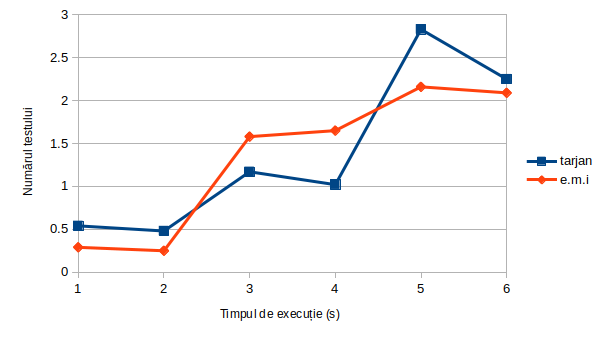
\includegraphics[width=10cm]{custom.png}
    \caption{Performanță pe testele speciale}
    \label{custom_teste}
\end{figure}

\subsection{Valori obținute}

Observăm că alg. cu determinarea E.M.I. își păstrează un nivel de performanță aproape constant în funcție doar de dimensiunea testelor, pe când alg. lui Tarjan depinde și de valorile din teste care influențează acele constante de timp. Dar pe testele unde avem mai multe interogări decât noduri, soluția cu păduri de mulțimi disjuncte prelevează.

Folosind utilitarul valgrind de pe sistemul de operare GNU/Linux, avem pe testul special 4, pentru implementarea cu E.M.I., \texttt{307,883,208} octeți de memorie alocată dinamic. Iar pentru cealaltă implementare, \texttt{106,316,252}.

Așadar, intuițiile noastre s-au confirmat în termeni de timp și memorie.

\section{Concluzii}

Deși reducerea problemei celui mai mic strămoș comun la determinarea elementului minim dintr-un interval, are cea mai bună performanță de timp, ceea ce ne demonstrează ingeniozitatea soluției propuse de Tarjan este flexibilitatea unei structuri de date care poate fi adaptată și altor nevoi, păstrând o logică arborescentă.

\newpage

\section{Algoritmi}

\begin{algorithm}
\caption{Soluția off-line a lui Tarjan}\label{tarjan}
\begin{algorithmic}[1]
\Procedure{$ocmmmsc$}{$nod$}
    \State \Call{\emph{formează\_mulțime}}{$nod$}
    \ForAll{$f\ fiu\ al\ lui\ nod$}
        \State \Call{$ocmmsc$}{$f$}
        \State \Call{\emph{unește}}{$f, nod$}
        \State \Call{\emph{marchează\_strămoș}}{$nod, nod$};
    \EndFor
    \State $nod.culoare \gets NEGRU$
    \ForAll{$nod\ v\ \textrm{a.î.}\ \{v, nod\} \in I$}
        \If {$v.culoare = NEGRU$}
            \State \textbf{$scrie$} \emph{"CMMSC de (" v "," nod ") ="} \Call{\emph{găsește\_mulțime}}{$v$}
        \EndIf
    \EndFor
\EndProcedure
\end{algorithmic}
\end{algorithm}

\begin{algorithm}
\caption{Algoritmul pentru tur eulerian}\label{tur_eulerian}
\begin{algorithmic}[1]
\Procedure{$tur\_eulerian$}{$nod, tur$}
    \State $nod.vizitat \gets$ \emph{adevărat}
    \State \Call{\emph{adaugă}}{$tur, nod$}
    \ForAll{$f\ fiu\ al\ lui\ nod$}
    	\If {$f.vizitat = fals$}
        	\State \Call{$tur\_eulerian$}{$f, tur$}
            \State \Call{\emph{adaugă}}{$tur, nod$}
        \EndIf
    \EndFor
\EndProcedure
\end{algorithmic}
\end{algorithm}

\newpage
\renewcommand{\refname}{Referințe}
\begin{thebibliography}{8}
\bibliographystyle{splncs04}

\bibitem{lca_taxonomie}
Kahlke, T., Ralph P.J.:  BASTA – Taxonomic classification of sequences and sequence bins using last common ancestor estimations. Methods in Ecology and Evolution \textbf{10}(1), 100--103 (2019).
\url{https://doi.org/10.1111/2041-210X.13095}

\bibitem{Harel_Tarjan}
Harel, D.; Tarjan, R. E.: Fast algorithms for finding nearest common ancestors. SIAM J. Comput. \textbf{13}(5), 338--355 (1984)

\bibitem{Teoria_Grafurilor}
Popescu, D.R.: Combinatorică și teoria grafurilor. Societatea de Științe Matematice din România, București (2005)

\bibitem{CLRS}
Cormen, T.H.; Leiserson, C.E.; Rivest, R.L.; Stein, C.: Introduction to Algorithms. 3rd edn. MIT Press and McGraw-Hill,
USA (2009)

\bibitem{lca_mostenire}
Stack Overflow Question, 
\url{https://stackoverflow.com/questions/15788725/how-to-determine-the-closest-common-ancestor-class}, 
Last accessed 1 Oct 2020

\bibitem{lca_algopedia}
Algopedia, Note de curs,
\url{http://algopedia.ro/wiki/index.php/Note_de_curs,_clasele_11-12,_13_martie_2014},
Last accessed 1 Oct 2020

\bibitem{lca_poza}
Wikimedia Foundation,
\url{https://commons.wikimedia.org/wiki/File:Lowest_common_ancestor.svg}, 
Last accessed 1 Oct 2020

\bibitem{infoarena_teste}
Infoarena,
\url{https://www.infoarena.ro/problema/lca?action=attach-list},
Last accessed 18 Dec 2020


\end{thebibliography}
\end{document}
